\section{Benchmarking}
\label{sec:benchmarking}


We present a set of experiments to evaluate the efficacy of the proposed
modular code generation tool (\ourTool) with \simulink.  In the first 
experiment, we evaluate the \emph{scalability} of \ourTool and \simulink as the 
number of cells in the \ac{NHN} model increases.  In the second experiment, we 
select benchmarks that span across different application domains such as 
medical, physics, and industrial automation to illustrate the \emph{diversity} 
of the proposed approach.  We compare each of these benchmarks against 
\simulink in terms of execution time and maximum memory usage.  


\subsection{Experimental set-up}
\label{sec:experimentalSetUp}
The following aspects were considered in order to achieve a fair
comparison between \ourTool and \simulink:

\begin{description}[\IEEEsetlabelwidth{Step Size}\IEEEusemathlabelsep]
\item[\textbf{Solver}] To reflect the synchronous execution model, we
  used a discrete numerical solver with a fixed step in \simulink,
  namely \texttt{ode1} (Forward Euler).
  
\item[\textbf{Step Size}] For all benchmarks the step size in \simulink
  is fixed to $0.01$ milliseconds.  The same step size is also used in
  \ourTool, $\delta = 0.01$ milliseconds.
  
\item[\textbf{Time}] All benchmarks were simulated for $10$ seconds of
  simulation time.  Based on a step size of $0.01$ milliseconds this
  translates to $1$ million iterations.
  
\item[\textbf{Compiler}] All code was compiled using the \compiler
  compiler.  \ourTool code was compiled using both no optimisation
  (\texttt{O0}) and \texttt{O2} optimisation.  \simulink code was
  compiled using the automatically generated Makefile.
\end{description}

The experiments were evaluated using an Intel~i7-4790 processor with
8~GB RAM on Windows~7.


\subsection{Scalability}

\begin{figure}[htbp]
  \centering
  \begin{tikzpicture}[yscale=0.85]
\begin{axis}
[
	xlabel={Number of Heart Nodes},
	ylabel={Execution Time ({s})},
	axis y line = left,
	axis x line = bottom,
	xmin=0000,
	xmax=1000,
	ymin=0,
	ymax=150,
	ytick={0, 10, 50, 100, 150},
	yticklabels={0, 10, 50, 100, 150},
	extra tick style={grid=major},
	legend style={
		at={(0.52,0.99)},
		anchor=north,
		legend columns=-1
	}
]

\addplot[color=blue!90,
	mark=square*,
	mark size=2
] table [
	x=n,
	y=s_t,
	col sep=comma
] {./figures/scalabilityGraphData.csv};
\addlegendentry{\simulink}

\addplot[color=red!90,
	mark=*,
	mark size=2
] table [
	x=n,
	y=p_t,
	col sep=comma
] {./figures/scalabilityGraphData.csv};
\addlegendentry{\ourTool}

\addplot[color=black!90,
	dashed,
	mark=.,
	mark size=2
] coordinates {
	(0,10)
	(1000,10)
} node[pos=0.8] (endofrealtime) {};
\node[above] at (endofrealtime) {Real Time};

\addplot[color=blue!90,
	dashed,
	mark=.,
	mark size=2
] coordinates {
	(297,126.448)
	(297,0)
};



\end{axis}
\end{tikzpicture}
  \caption{Scalability in  execution time of \simulink and \ourTool against 
  number of nodes in the \acf{NHN} model.}
  \label{fig:scalability}
\end{figure}

For the purposes of this experiment we aim to validate the scalability of
\ourTool through the running example of the \ac{NHN} whilst comparing it
to \simulink.  Code was generated for varying network sizes ($33$ cells,
$66$ cells, $99$ cells, etc.) and the execution time recorded.  The
experimental set-up was the same as described in
Section~\ref{sec:experimentalSetUp}, ie. $1$ million iterations at a
$0.01$ millisecond step size.

The results are shown in Figure~\ref{fig:scalability}, with the most
obvious feature being that no data is recorded for \simulink for
complexities greater than $297$ cells.  \simulink imposes an inbuilt
requirement that the generated code use less than $2$GB of memory. This
discontinuity represents the point after which the memory usage exceeds
this limit.\footnote{\simulink memory usage at a $297$ cell network is
  $1.8$GB.}  \ourTool, on the other hand, is able to continue past this
point.

These results also illustrate that \ourTool has a smaller increase in
Execution Time as network size increases meaning that it is able to
maintain real-time with a model roughly $5$ times larger ($200$ cells vs
$40$ cells) than \simulink.  It is also of note that the change in
gradient of \ourTool around the $200$ cell mark is due to the memory
usage exceeding the L$3$ cache size ($8$MB in our CPU).


\subsection{Diversity}
\label{sec:diversity}

\begin{figure}[htbp]
  \centering
  \subfigure[Execution time relative to \simulink \label{fig:executionTime}]{
    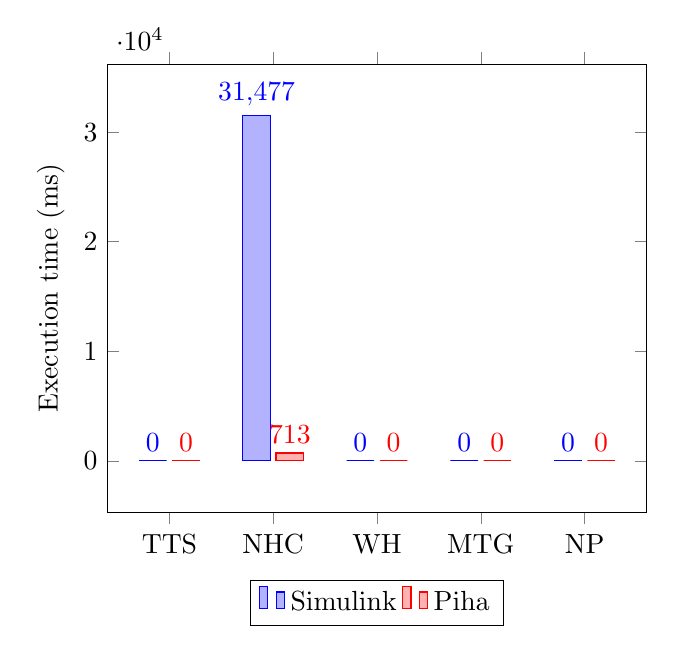
\begin{tikzpicture}
\begin{axis}[
	ybar,
	enlargelimits=0.15,
	legend style={
		at={(0.5,-0.15)},
		anchor=north,
		legend columns=-1
	},
	ylabel={Execution time (ms)},
	symbolic x coords={TTS, NHC, WH, MTG, NP},
	xtick=data,
	nodes near coords,
	nodes near coords align={vertical},
]

%Simulink
\addplot coordinates {
	(TTS,0)
	(NHC,31477)
	(WH,0)
	(MTG,0)
	(NP,0)
};

%Piha
\addplot coordinates {
	(TTS,0)
	(NHC,713)
	(WH,0)
	(MTG,0)
	(NP,0)
};

\legend{Simulink, Piha}

\end{axis}
\end{tikzpicture}

  }
  \subfigure[Executable size (KB) \label{fig:executableSize}]{
    \begin{tikzpicture}
\begin{axis}[
	ybar,
	width=\linewidth-5mm,
	height=5cm,
	enlarge y limits={upper, value=0.1},
	enlarge x limits=0.15,
	legend style={
		at={(0.5,1.15)},
		anchor=north,
		legend columns=-1
	},
	ylabel={Executable Size (KB)},
	ymin=0,
	symbolic x coords={TSN, NHN, WH, MTG, NP},
	xtick=data,
%	nodes near coords,
	nodes near coords align={vertical},
]

%Simulink
\addplot coordinates {
	(TSN,190)
	(NHN,320)
	(WH,226)
	(MTG,188)
	(NP,212)
};

%Piha (O0)
\addplot coordinates {
	(TSN,131)
	(NHN,323)
	(WH,163)
	(MTG,130)
	(NP,174)
};

%Piha (O2)
\addplot coordinates {
	(TSN,96)
	(NHN,128)
	(WH,98)
	(MTG,97)
	(NP,98)
};


\legend{\simulink, \ourTool (O0), \ourTool (O2)}

\end{axis}
\end{tikzpicture}

  }
  \caption{Comparison of the execution time (in ms) and executable size
    (in KB) between \simulink and \ourTool for the benchmarks in
    Table~\ref{tab:benchmarks}.}
  \label{fig:results}
\end{figure}

The purpose of the second experiment, we use the five benchmarks
presented in Table~\ref{tab:benchmarks}.  The table also presents the
number of locations (\#L) in each hybrid automata.  For example,
$(2^{50})$ denotes that the \acf{TSN} benchmark is described by $50$
instances of an \ac{HIOA} with two locations.

For all the benchmarks, the executable for the \simulink models are
generated using the in-built Real-time
Workshop\textsuperscript{\textregistered} C code generator.  Similarly,
for \ourTool, we generate equivalent C code, and compile it using a
standard C compiler.
The execution times and executable sizes of the generated programs are reported below and illustrated in Figure~\ref{fig:results}.\\

\textbf{Execution time:} Figure~\ref{fig:executionTime} shows that for
all benchmarks the execution time of \ourTool (both with no optimisation
and with optimisation level \texttt{O2}) is faster than that of
\simulink.  On average, we show that \ourTool is $9.8$ times faster than
\simulink.
For our most complicated example, the \ac{NHN}, we observe an improvement of 
$20.3$ times.\\

\textbf{Code size:} Figure~\ref{fig:executableSize} shows that the code
generated by \ourTool is also, generally, more compact than that
generated by \simulink.  On average, the optimised code of \ourTool is
$54\%$ smaller than \simulink when compiled.
For the \ac{NHN} example, the unoptimised code of \ourTool is comparable to 
that of \simulink while the optimised code sees improvements similar to that of 
the other benchmarks.\\

In summary, the code generated by \ourTool executes $9.8$ times faster
on average, with the executable size being $54\%$ smaller on average
when compared to \simulink.  \ \begin{table*}
	\centering
	\caption{Benchmark descriptions
	\label{tab:benchmarks}}
\begin{tabular}{ | c | c | c | l | } \hline
\textbf{Benchmarks}
	& \textbf{Domain} 
	& \textbf{\#L } 
	& \textbf{Description} \\ \hline

	\acf{TTS}
		& Physics~\cite{Pedro2005}
		& $(2, 2, 2)$
		& Three thermostats heating a room to keep it warm\\ \hline
		
	\acf{NHC}
		& Biology~\cite{chen201487}
		& $(4^{33})$
		& Captures the electrical conduction system of a heart with $33$ nodes\\ \hline

	\acf{WH}
		& Physics~\cite{raskin05}
		& $(4, 4)$
		& Models the heating of water in a tank \\ \hline
		
	\acf{MTG}  
		& Industrial automation~\cite{Costello2013}
		& $(2, 3^{30})$
		& Models the behaviour of a gate and $30$ trains at a rail road crossing\\ \hline
		
	\acf{NP}
		& Industrial automation~\cite{alur2015book}
		& $(3^{30}, 3^{30})$
		& Switches between two fuel rods in 30 reactors to avoid nuclear meltdown\\ \hline
	
	
 \end{tabular}
 \end{table*}


%%% Local Variables:
%%% mode: latex
%%% TeX-master: "../DATE2016_codegen"
%%% End:
